\documentclass[11pt]{amsart}
\usepackage[T1]{fontenc}
\usepackage[utf8]{inputenc}
\usepackage{lmodern,amsmath,amssymb,amsthm,mathtools,microtype,graphicx}
\usepackage[a4paper,margin=25mm]{geometry}
\usepackage[hidelinks]{hyperref}
\usepackage{xurl}
\newtheorem{theorem}{Theorem}[section]
\newtheorem{lemma}[theorem]{Lemma}
\newtheorem{proposition}[theorem]{Proposition}
\newtheorem{corollary}[theorem]{Corollary}
\theoremstyle{remark}\newtheorem{remark}[theorem]{Remark}
\newcommand{\Z}{\mathbb Z}\newcommand{\Q}{\mathbb Q}\newcommand{\F}{\mathbb F}
\newcommand{\oo}{\mathfrak o}\newcommand{\NN}{\mathcal N}
\newcommand{\OO}{\mathcal O}\newcommand{\SSS}{\widehat{\mathcal S}}
\newcommand{\vp}{v_p}\newcommand{\Disc}{\operatorname{Disc}}
\newcommand{\Spec}{\operatorname{Spec}}\newcommand{\diag}{\operatorname{diag}}
\newcommand{\Span}{\operatorname{span}}\newcommand{\length}{\operatorname{length}}
\newcommand{\im}{\operatorname{im}}\newcommand{\supp}{\operatorname{supp}}
\newcommand{\Leg}[2]{\left(\frac{#1}{#2}\right)}
\allowdisplaybreaks

\title{Two integral degeneration types of the signed Erd\H{o}s--Straus quartic}
\author{The Clankers}
\date{20 September 2026}
\begin{document}
\begin{abstract}
We specialize the finite signed completion of the literal-root ES quartic at its
original prime. Its integral normalization index is $p^2$ for Type I and $p^9$
for Type II, despite constant rank eight. The original coordinate conductors,
Smith factors and generic rational-point counts are explicit. The new Type-I
boundary point lifts modulo $p^2$ but never modulo $p^3$. These statements
compare original arithmetic states; they do not prove an ES state exists at
every prime.
\end{abstract}
\maketitle

\begin{figure}[htbp]
\centering
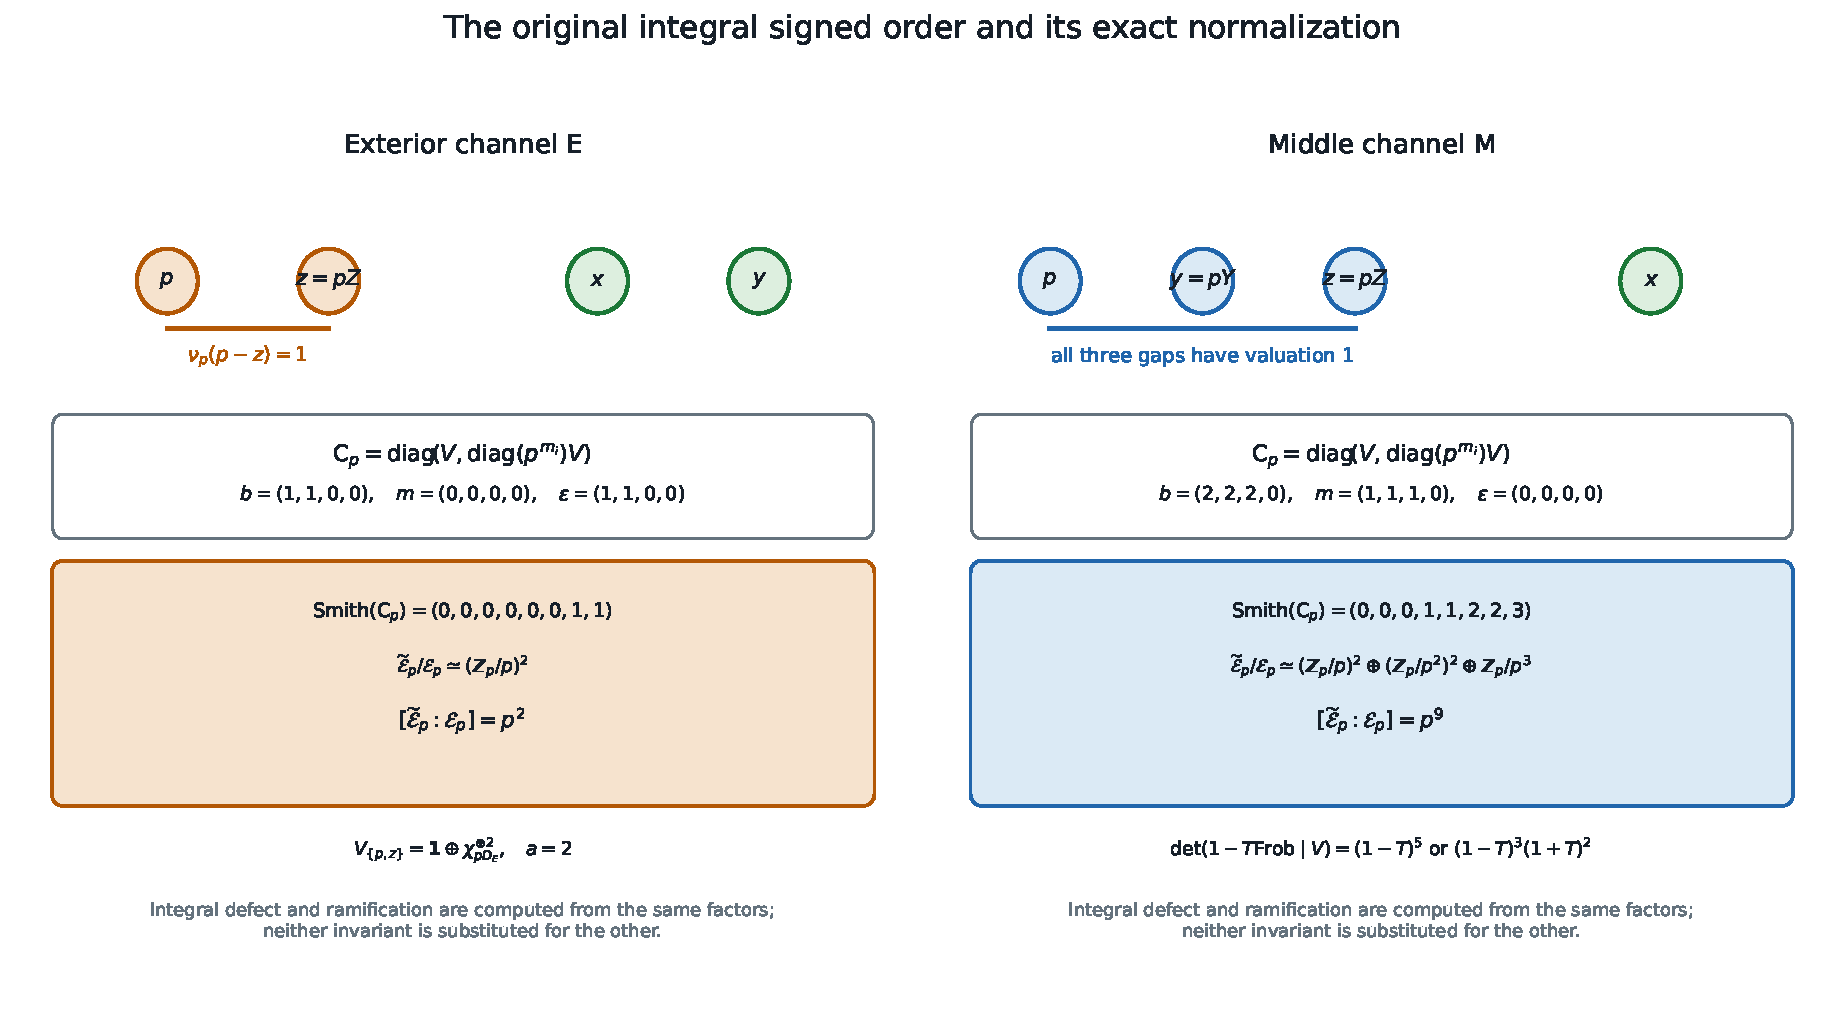
\includegraphics[width=\textwidth]{figures/integral-normalization-smith.pdf}
\caption{The exact normalization matrix in the original ordered basis.  Its
Smith exponents give index $p^2$ in Type I and $p^9$ in Type II; the complete
matrix proof and conductor ideals follow below.}
\end{figure}

\section{The original source and its finite signed completion}
Let $p\equiv1\pmod{12}$ be prime. Retain $p/4<a<p/2$, $R=4a-p$, $u\mid a^2$,
and either $E:R\mid4u+1$ or $M:R\mid u+a$. With
\[
 d=\gcd(a,u),\quad(h,r,s)=(d^2/u,u/d,a/d),
\]
the original Type-I/II denominators are
\[
 E:(a,hs\kappa,phr\kappa),\quad\kappa=(pr+s)/R;
 \qquad M:(a,phs\lambda,phr\lambda),\quad\lambda=(r+s)/R.
\]
These inherited coordinates \cite[\S2]{ET} retain $a=hrs$, $u=hr^2$ and
$\gcd(r,s)=1$. The ordered inverses are $a^2/(Ry-pa)$ and $pa^2/(Ry-pa)$.
Reciprocity gives $(l/R)=(l/p)$ for every prime $l\mid a$, including two by the
supplementary law. Hence
\[
 E:(h/p)=-1,\qquad M:(rs/p)=-1.                         \tag{1}
\]
The M claim uses $r\equiv-s\pmod R$.

Set $\oo=\Z_p$, $K=\Q_p$, and retain the literal ordered roots
\[
 (\ell_0,\ell_1,\ell_2,\ell_3)=(p,x,y,z),\quad
 S=p+x+y+z,\quad H(T)=-S^{-1}\prod_i(T-\ell_i).
\]
The cubic coefficient of $H$ is one. The given signed-completion construction
\cite[\S3, (18)--(24)]{Input} is
\[
 \widehat S=\oo[T,\eta]/(H,\eta^2-H'),                   \tag{2}
\]
with original basis $1,T,T^2,T^3,\eta,\eta T,\eta T^2,\eta T^3$.
It recovers the original affine inverse only on $\eta\ne0$, with $\xi=\eta^{-1}$.
We prove below that $S$ is a $p$-unit, so (2) is indeed finite free of rank eight
over this original arithmetic ring.

For E write $(x,y,z)=(a,b,pc)$. The original identity
$p\mathsf D+1=4hr\kappa$ gives $c\equiv1/4\pmod p$.
Both $a-b=hs(r-\kappa)$ and $a+b=hs(r+\kappa)$ are units: the contrary would
make the nonresidue $hr^2$ equal to $1/4$ or $-1/4$ modulo $p$. Thus only
$\ell_0,\ell_3$ have a nonunit difference, of valuation one, and $S\equiv a+b$.

For M write $(x,y,z)=(a,pb,pc)$. Here $b,c$ are units,
$4bc\equiv b+c$, and $(bc/p)=-1$ by (1). They are distinct modulo $p$ because
$r,s<p$ are distinct. Neither is one: then the other would be $1/3$, contrary
to $(3/p)=1$. Thus the cluster $\ell_0,\ell_2,\ell_3$ has all pair differences
of valuation one, its singleton $a$ is separated by units, and $S\equiv a$.

Writing $d_i=H'(\ell_i)$, we have therefore proved
\[
 E:\ (v_p(d_i))=(1,0,0,1),\qquad
 M:\ (v_p(d_i))=(2,0,2,2).                              \tag{3}
\]

\section{Complete normalization and conductor}
Let $k_i=\lfloor v_p(d_i)/2\rfloor$ and
\[
 N_i=\oo[\theta_i]/(\theta_i^2-d_i/p^{2k_i}),\qquad
 N=\prod_iN_i.
\]
Each $N_i$ is maximal: its quadratic is either a split unit quadratic, an
unramified unit quadratic, or an Eisenstein quadratic of odd residue
characteristic. A direct proof is obtained by taking trace and norm of
$a+b\theta_i$: trace forces $a\in\oo$, then norm forces $b\in\oo$.
In the split case use the two values and the unit $2\sqrt{d_i/p^{2k_i}}$.
The exact normalization map is
\[
 f(T)+\eta g(T)\longmapsto
 \bigl(f(\ell_i)+p^{k_i}g(\ell_i)\theta_i\bigr)_i.        \tag{4}
\]

\begin{theorem}
For Type I,
\[
 N/\widehat S\simeq(\oo/p)^2,
 \qquad\mathfrak f=pN_0\times N_1\times N_2\times pN_3.
\]
For Type II,
\[
 N/\widehat S\simeq(\oo/p)^2\oplus(\oo/p^2)^2\oplus\oo/p^3,
 \qquad\mathfrak f=p^3N_0\times N_1\times p^3N_2\times p^3N_3.
\]
Thus the normalization indices are $p^2$ and $p^9$, respectively.
\end{theorem}
\begin{proof}
Unit resultants split off the noncolliding root factors integrally. For E the
remaining root lattice is
$L_2=\{(v_0,v_3):v_0\equiv v_3\pmod p\}$, by linear interpolation across a
root difference of exact valuation one. Its Smith factors are $1,p$.
Equation (4) gives $L_2\oplus L_2$, and four already maximal outside coordinates.
A normal value supported at one cluster root belongs to the order precisely
when both its coefficients in $1,\theta_i$ are divisible by $p$. This gives the
quotient and maximal conductor ideal in the Type-I case.

For M use the Newton basis $1,T-p,(T-p)(T-pb)$ on the three clustered roots.
Evaluation has Smith factors $1,p,p^2$, so its root lattice $L_3$ has index
$p^3$. Equation (4) gives $L_3\oplus pL_3$, with exponents $(0,1,2,1,2,3)$,
and two outside zeros. A value $a+b\theta_i$ supported at one cluster root has
Lagrange denominators of order $p^2$. Thus membership requires
$a\in p^2\oo,b\in p^3\oo$. Membership after multiplication by the unit
$\theta_i$ forces both into $p^3\oo$. That condition is also sufficient, proving
the Type-II conductor and quotient.
\end{proof}

In particular the eight Smith exponents are
\[
 (0,0,0,0,0,0,1,1)\quad\hbox{and}\quad(0,0,0,1,1,2,2,3).
\]
The full inverse of (4) interpolates the values $a_i$ and $b_i/p^{k_i}$
separately. It is integral exactly when all eight original polynomial
coefficients are integral. The nonzero finite quotient is retained; no
$\oo$-linear section from that torsion quotient into the torsion-free $N$ exists.
These conductors are conductors of finite orders, not the analytic weighted
conductor used elsewhere in the programme.

\section{Generic signed points and special boundary points}
Over $K$, (2) is $\prod_iK[\eta_i]/(\eta_i^2-d_i)$.
For E the two valuation-one square classes are equal, because their unit ratio
is $-1\pmod p$. At the other two roots the derivative residues are
$-a^2(a-b)/(a+b)$ and $-b^2(b-a)/(a+b)$, also with square ratio. Thus the fibre
has either four $K$-points or none; its nonsplit factors are two copies of a
ramified quadratic and possibly two copies of an unramified quadratic.
For M, the singleton derivative is $-a^2\pmod p$. The three cluster derivatives
after division by $p^2$ have residues
\[
 (1-b)(1-c),\quad(b-1)(b-c),\quad(c-1)(c-b).
\]
Their product is a negative square. Either all three or exactly one is square,
so the complete fibre has eight or four $K$-points. Unit square roots lift by
$z_{n+1}=z_n-p^n((z_n^2-d)/p^n)(2z_n)^{-1}\pmod{p^{n+1}}$.
This accounts for every signed point and every field factor.

The colliding special blocks are respectively
\[
 \F_p[\eta]/\eta^4,
 \qquad
 \F_p[\epsilon,\eta]/(\epsilon^3,\eta^2-3\epsilon^2).
\]
Their lengths are four and six, while multiplication by $\eta$ has Jordan blocks
$(4)$ and $(4,2)$. The original inverse obtained by inverting $\eta$ deletes
these entire nonzero local blocks; it does not make their poles finite.

\begin{theorem}
The added Type-I point $(T,\eta)=(0,0)\pmod p$ has exactly $p$ lifts modulo
$p^2$, but no lift modulo $p^3$.
\end{theorem}
\begin{proof}
Factor $H(T)=U(T)(T-p)(T-pc)$, where $U(0)=-ab/S$ is a unit and $c=1/4\pmod p$.
For $T=pw,\eta=pv$, the root equation is automatic modulo $p^2$, and the
quadratic equation requires $2w-1-c=0\pmod p$. Thus $w=5/8$ and all $p$ choices
of $v$ work. But every next lift has
\[
 H(T)/p^2\equiv-U(0)(1-c)^2/4=9ab/(64S)\ne0\pmod p.
\]
The root equation fails already modulo $p^3$.
\end{proof}

At the hard prime $1009$, the original E denominators
$(253,87032,3818056)$ have \emph{no} $K$-rational signed inverse, while the
original M denominators $(253,2042216,88792)$ have eight. Both are positive
integer ES identities. Thus degree-eight finite flatness is not rational-point
or integral-section surjectivity. The proper map retains length at its boundary;
it does not discharge the prime-by-prime original occupancy problem.

The distinguished-prime idempotent
\[
 e_p(T)=\frac{\prod_{i=1}^3(T-\ell_i)}{\prod_{i=1}^3(p-\ell_i)}
\]
has an exact denominator $p$ in E and $p^2$ in M. Hence the generic prime-only
sign map $\eta\mapsto(1-2e_p)\eta$ does not preserve the original integral
order, whereas the global sign does. Both extend to the normalization. This
states the actual loss instead of deleting the original prime-root marking.

\section{Provenance and execution boundary}
The literal target, finite rank-eight extension and open inverse are supplied
antecedents \cite{Input}. The indices, original conductors, local signed types,
and sharp finite lifting obstruction are derived here. No historical-priority
claim is made. The full companion proof gives all coordinate maps, the reciprocal
quadratic twist, and explicit finite-place rational controls satisfying the
supplied height inequalities but missing one global denominator condition.
It also transports the previously proved $p=825241$ capacity crossing; that
crossing is supplied by original divisor arithmetic, not by assuming an inverse
point of this finite cover.

The package's standard-library verifier and a separate primitive-source checker
compare every labelled E/M state at all primes $p\equiv1\pmod{12}$ through 3000.
The detailed original lattice and inverse examples, finite special fibres,
negative controls and command receipts are included. Finite replay does not
prove initial ES occupancy, a Lean build or an independent mathematical review.
\begin{thebibliography}{9}
\bibitem{ET} C.~Elsholtz and T.~Tao (2013), \emph{Counting the number of solutions
to the Erd\H{o}s--Straus equation on unit fractions}, J. Aust. Math. Soc. 94,
50--105, \S2. \url{https://arxiv.org/abs/1107.1010}.
\bibitem{Input} The Clankers / Split-Zero continuation (2026), supplied
\texttt{Pasted markdown(20260920-025519).md}, \S\S1--3, especially equations
(8)--(11) and (18)--(24). Original source preserved with this package.
\end{thebibliography}
\end{document}
